%****************************************************************************************************************
\section{Introducción}
\subsection{Motivación}
\begin{frame}
	\frametitle{Motivación}
	\begin{block}{}
		
	\end{block}
\end{frame}

%================================================================================================================
\subsection{Sintonización de Controladores}
\begin{frame}[shrink=20]{Sintonización de Controladores}
	\begin{figure}
		\begin{center}
			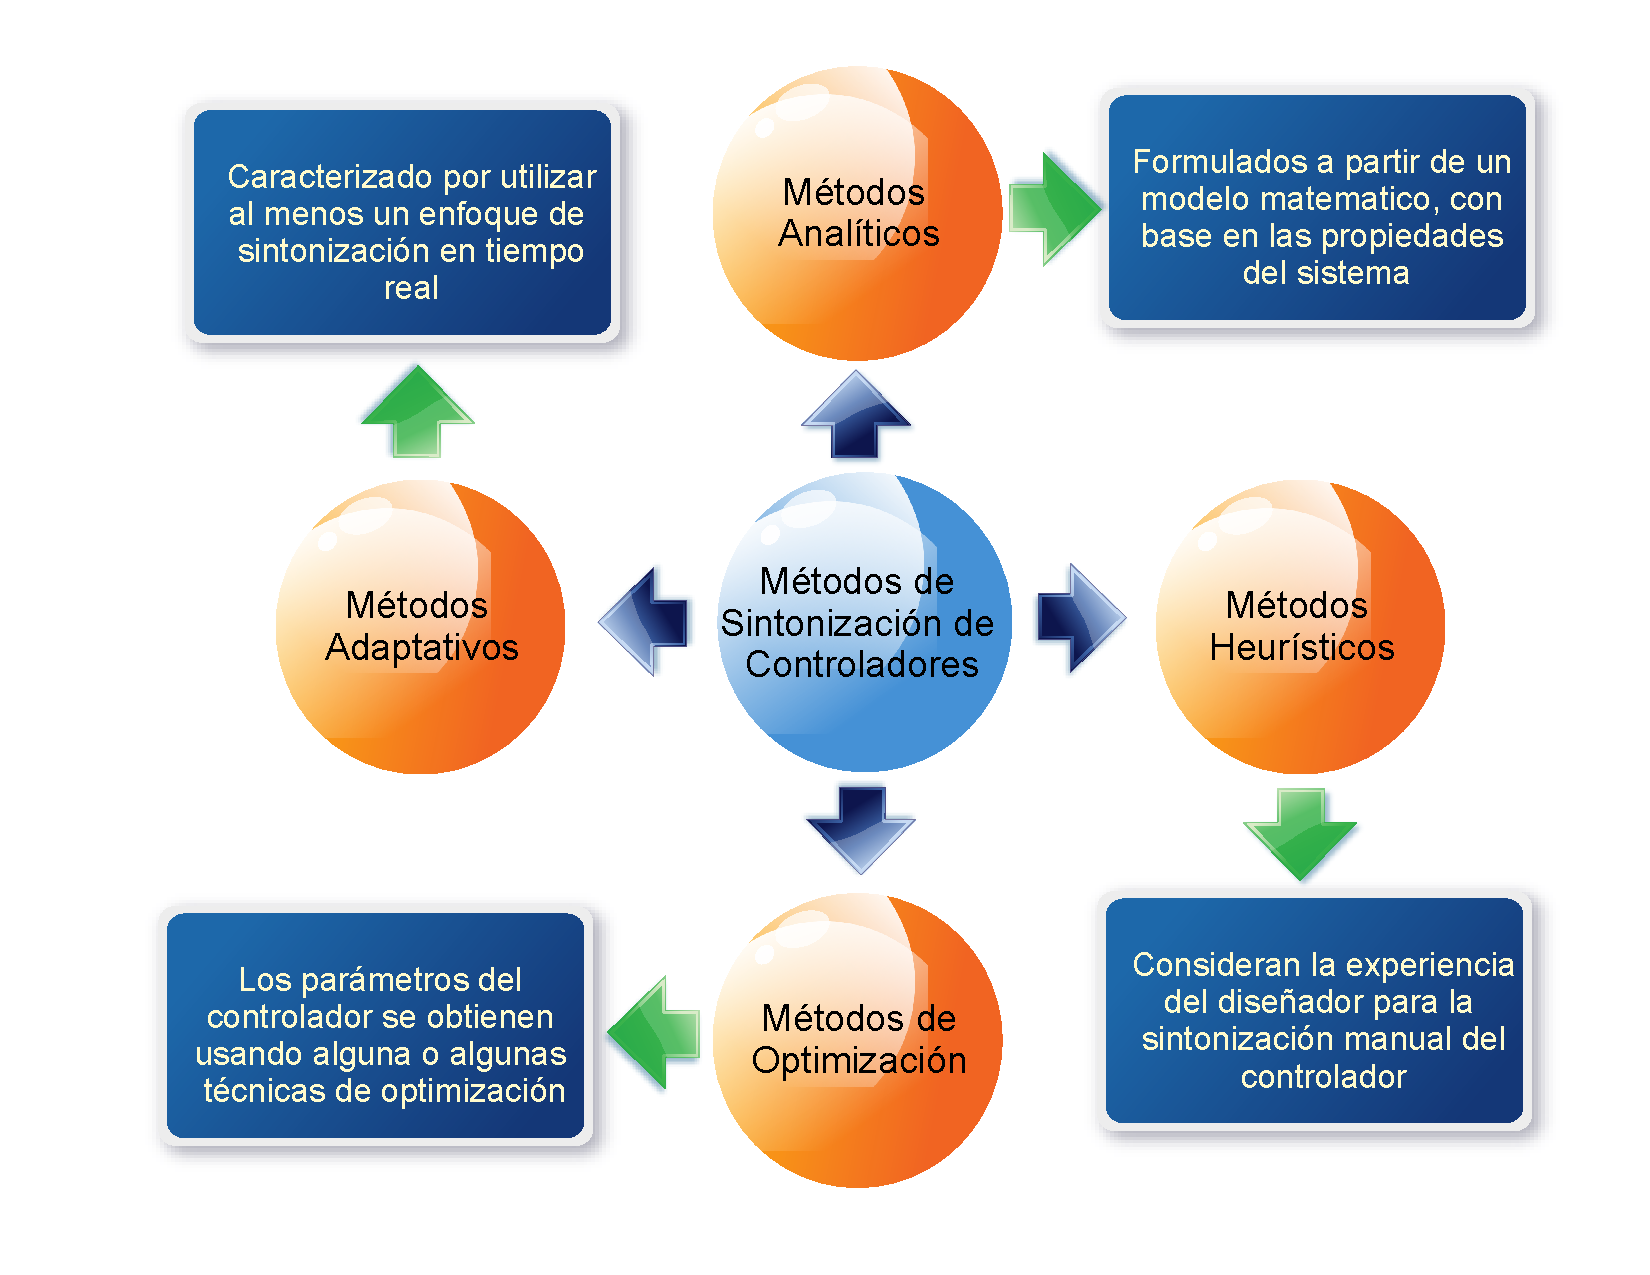
\includegraphics[scale=1]{Introduccion/MetSintCtrl.pdf}  
		\end{center}
	\end{figure}

\end{frame}

%================================================================================================================
\subsection{Paradigmas del control por computadora}
\begin{frame}[shrink=30]{Paradigmas de control por computadora}
	\begin{block}{Control disparado por tiempo}
		\begin{figure}
			\begin{center}
				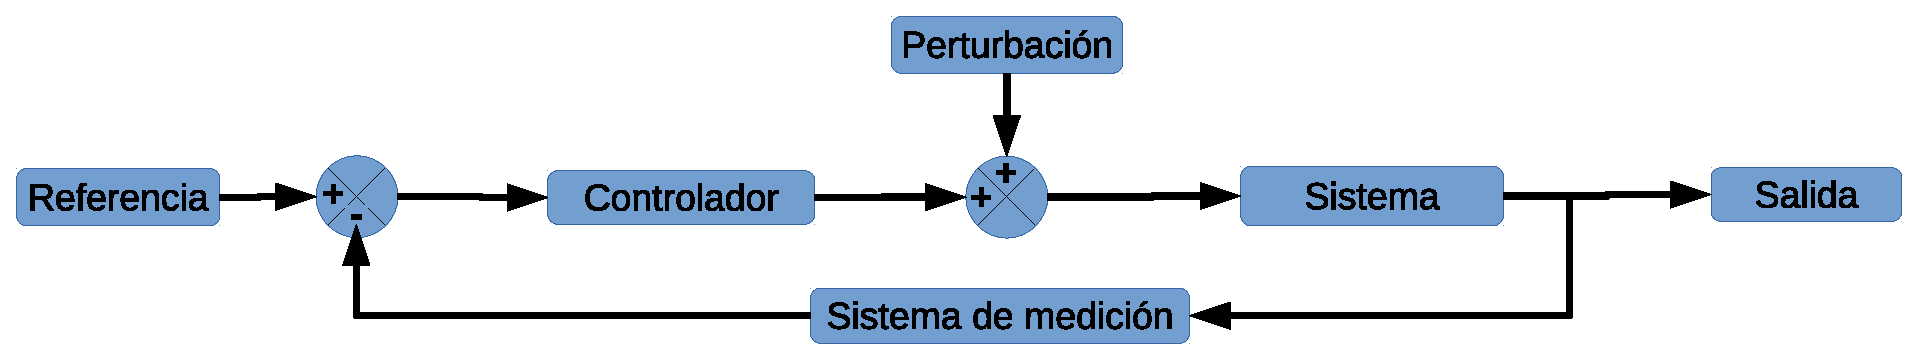
\includegraphics[scale=0.35]{Introduccion/EsqCtrlDispTiempCont.eps}
			\end{center}
		\end{figure}
		\begin{figure}
			\begin{center}
				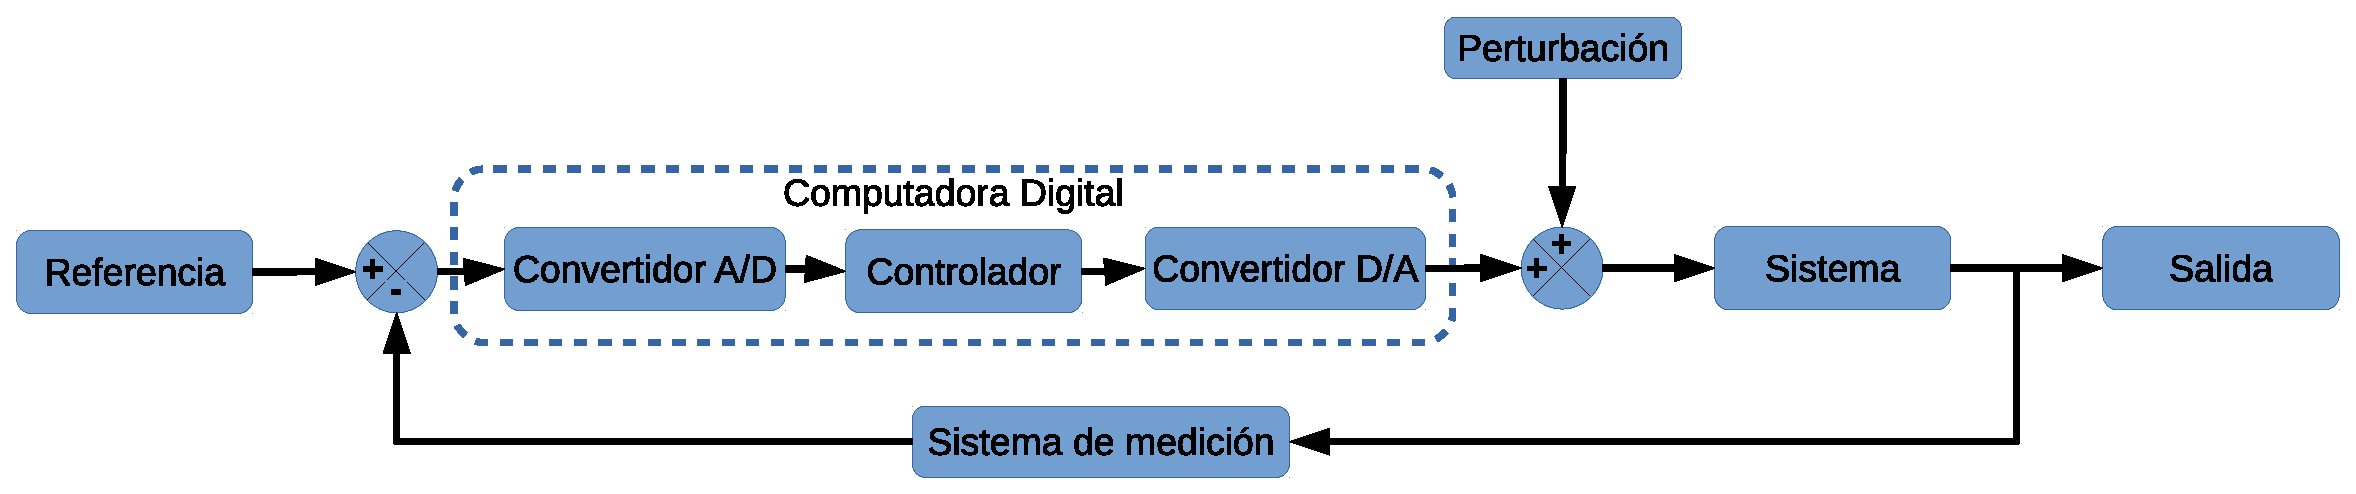
\includegraphics[scale=0.35]{Introduccion/EsqCtrlDispTiempDisc.eps} 
			\end{center}
		\end{figure}
	\end{block}
	\begin{block}{Control disparado por eventos}
		\begin{figure}
			\begin{center}
				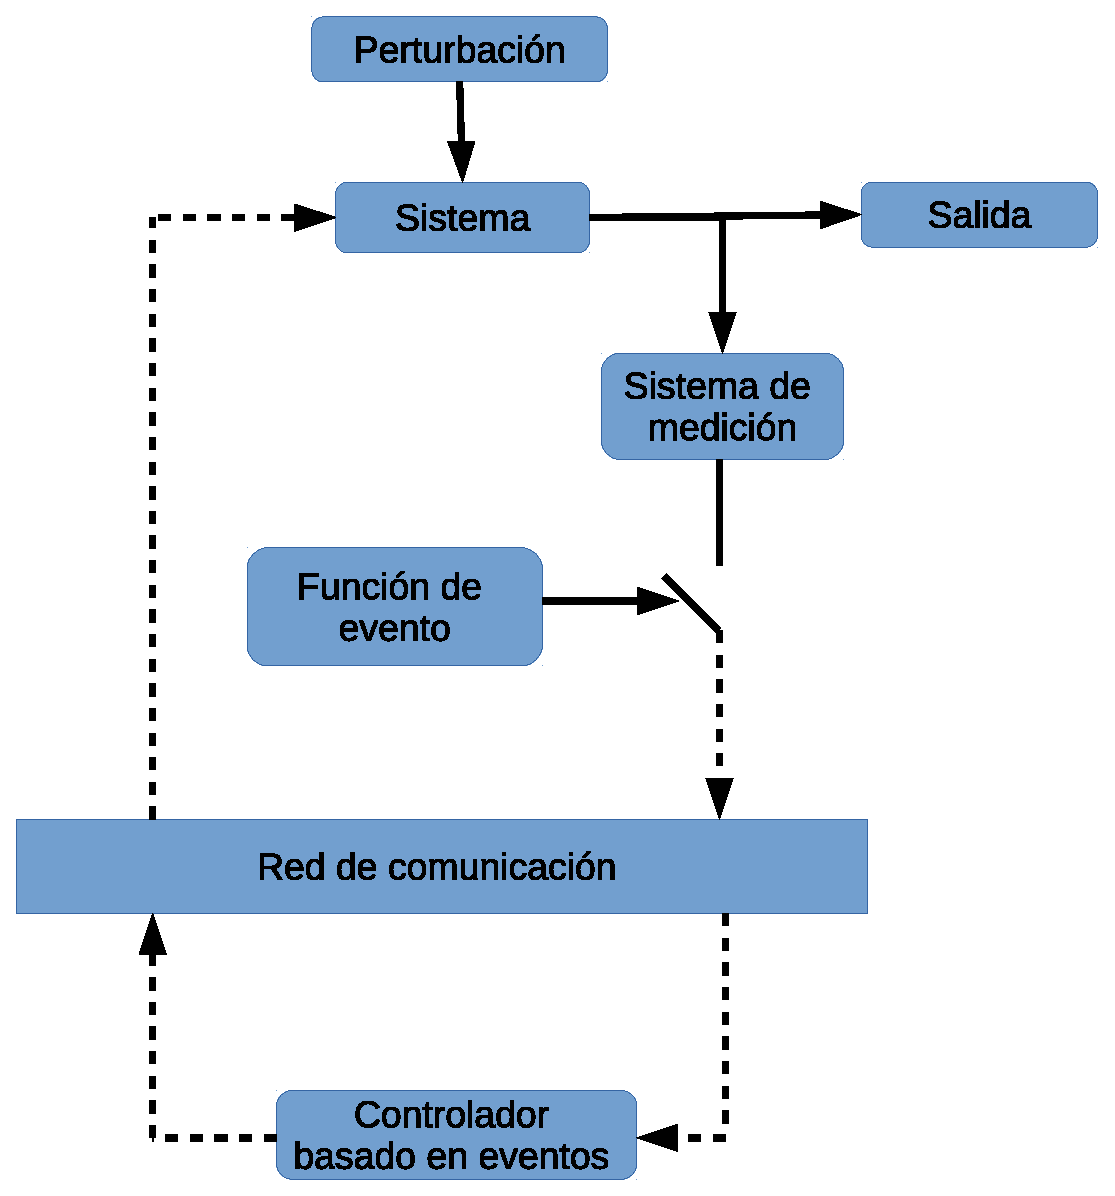
\includegraphics[scale=0.35]{Introduccion/EsqCtrlDispEvent.eps}  
			\end{center}
		\end{figure}
	\end{block}
\end{frame}

%================================================================================================================
\subsection{Planteamiento del Problema}
\begin{frame}[shrink=20]{Planteamiento del Problema}
\begin{block}{}
	\justifying
	Actualmente el desarrollo de controladores disparado por eventos a ido en aumento debido a que su rendimiento no se ve afectado en comparación con los controladores disparados por tiempo. Por otro lado los controladores disparados por eventos presentan la ventaja de disminuir en gran medida la carga computacional en comparación con los controladores disparados por tiempo. Sin embargo durante el diseño de los controladores disparados por eventos no se asegura una convergencia del error a cero en un tiempo establecido, sólo se garantiza cuando el tiempo tiende a infinito.
	
	Por lo anterior, en el presente trabajo se plantea como un problema de optimización, la sintonización de un controlador disparado por eventos abordando el problema de regulación para un robot manipulador. Bajo este enfoque se busca minimizar el tiempo de convergencia del error cuando este tiende a cero. Debido a la naturaleza del controlador disparado por eventos, se propone como evento de activación del controlador un intervalo de error, que cambiará según la aplicación.
\end{block}
\end{frame}

%================================================================================================================
\subsection{Objetivos}
\begin{frame}[shrink=20]{Objetivos}
\begin{block}{Objetivo general}
	\begin{itemize}
		\justifying
		\item Actualizar de forma óptima la señal de control generada a partir del enfoque de control disparado por evento con el propósito de garantizar un desempeño apropiado en la realización de tareas desarrolladas por un robot manipulador.
	\end{itemize}
\end{block}
\begin{block}{Objetivos particulares}
	\justifying
	\begin{itemize}
		\item Desarrollar el enfoque de control basado en eventos en un robot manipulador de tres grados de libertad.
		\item Establecer el problema de optimización que resuelve el objetivo general del proyecto.
		\item Resolver el problema con alguna técnica de optimización.
	\end{itemize}
\end{block}
\end{frame}

%================================================================================================================
\subsection{Justificación}
\begin{frame}[shrink=20]{Justificación}
\begin{block}{}
	\justifying
	La demanda de sistemas mecatrónicos que presenten una mejor eficiencia energética cada día va en aumento debido a la necesidad de disminuir costos de operación. Por tal motivo la aplicación de un enfoque de control disparado por eventos en un robot manipulador asegura una disminución en la carga computacional y a su vez disminuye el consumo energético, lo que en consecuencia produce un menor costo. Este enfoque depende en gran medida de la apropiada sintonización de sus parámetros, por tal motivo la importancia de este trabajo de investigación radica en la sintonización de los parámetros de un controlador disparado por eventos para un robot manipulador, de tal manera que el sistema presente un rendimiento aceptable bajo un tiempo y margen de error deseados.
\end{block} 
\end{frame}

%================================================================================================================
\subsection{Metodología} 
\begin{frame}[shrink=20]{Metodología}
%	\vskip0.5cm
	\begin{block}{Metas semestre B17} 			
		\justifying		
		\begin{itemize}
			\item [I)] Obtención del modelo dinámico del robot manipulador.
			\item [II)] Planteamiento y desarrollo del controlador disparado por eventos.
			\item [III)] Puesta en marcha del prototipo experimental.
			\item [IV)] Escritura formal obtención y formulación modelo dinámico y del controlador propuesto.
			\item [V)] Formulación del problema de optimización.
		\end{itemize}
	\end{block}
		\begin{block}{Metas semestre A18} 			
		\justifying		
		\begin{itemize}
			\item [VI)] Resolución del problema de optimización bajo alguna técnica de optimización.
			\item [VII)] Validación del los resultados de forma numérica.
			\item [VIII)] Divulgación del trabajo de investigación en congresos o revistas nacionales o internacionales.  
			\item [IX)] Escritura de los resultados del problema de optimización y su solución.
		\end{itemize}
	\end{block}
		\begin{block}{Metas semestre B18} 			
		\justifying		
		\begin{itemize}
			\item [X)] Validación de resultados de forma experimental.
			\item [XI)] Escritura de los resultados experimentales y terminación del documento de tesis.
			\item [XII)] Presentación del trabajo de tesis.
		\end{itemize}
	\end{block}

\end{frame}